En este capítulo se presentarán los detalles de diseño del proyecto, basándonos
en el análisis mostrado en el capítulo anterior. El modelo de clases de diseño
representado aquí es más fiel a la implementación final que el diagrama de
clases conceptuales, pero aún así hay detalles que no se han contemplado por ser
demasiado cercanos a los detalles de implementación.

También en el presente capítulo se detallarán las decisiones de diseño en
relación al aspecto visual de la aplicación, extendiéndonos en el proceso de
creación del logotipo del juego así como de la interfaz gráfica de usuario.

\section{Diagrama de clases de diseño}

Tras la fase de diseño, componían el sistema más de 40 clases, por lo que hemos
tenido que dividir los diagramas en varias partes, intentando seguir cierto
criterio a la hora de elegir qué clases formarán parte de cada división.

En todos los diagramas aparecen, en aras de mantener el contexto, las clases
básicas de la aplicación: \textit{Juego} y \textit{Estado}. Además, hay algunas
otras clases que también se repetirán entre diagramas por conveniencia. Para
mantener la legibilidad, se han ocultado los miembros privados y protegidos.

\begin{itemize}
\item En el primer diagrama (figura~\ref{fig:diagrama_clases_1}) aparecen las clases
  relacionadas con el \textit{menú principal}, clases de utilidades (logging y
  animación), y clases para representar elementos gráficos.
\item En el segundo diagrama (figura~\ref{fig:diagrama_clases_2}) aparecen las
  clases relacionadas con el subsistema de análisis del audio, así como las
  secciones \textit{Analizador de Notas} y \textit{Calibrar micrófono}.
\item En el tercer diagrama (figura~\ref{fig:diagrama_clases_3}) aparecen todas las
  clases relacionadas con la sección de \textit{Canciones}.
\item En el cuarto y último diagrama (figura~\ref{fig:diagrama_clases_4}) aparecen
  las clases relacionadas con el motor de \textit{lecciones}.
\end{itemize}

\begin{figure}[htp!]
  \centering
  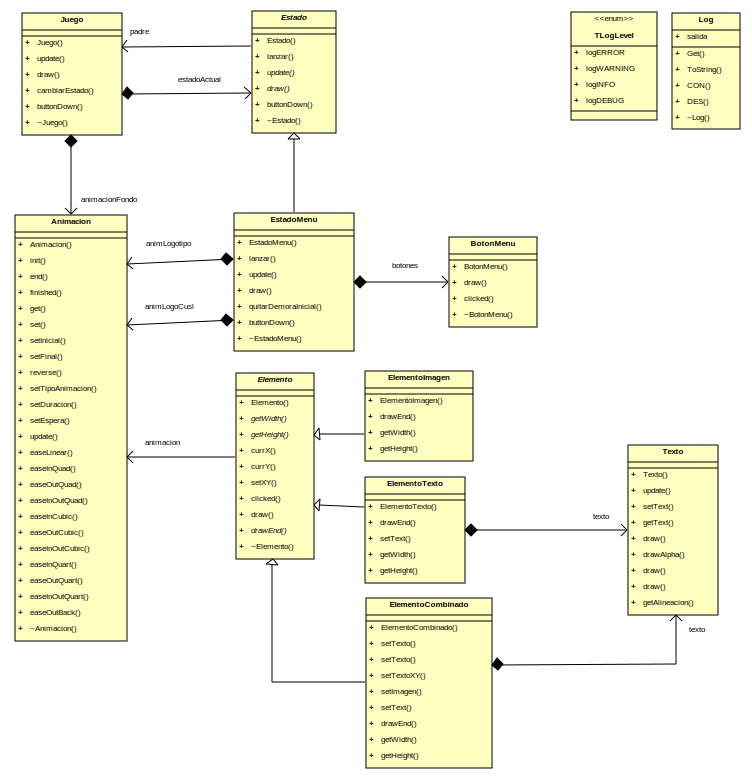
\includegraphics[width=\textwidth]{5_diseno/diagrama1}
  \caption{Diagrama de clases de diseño, parte I}
  \label{fig:diagrama_clases_1}
\end{figure}

\begin{figure}[htp!]
  \centering
  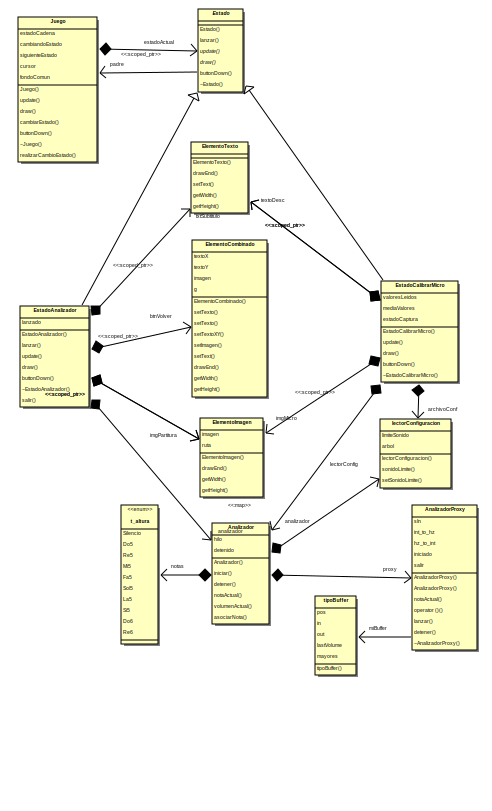
\includegraphics[width=\textwidth, clip=true, trim=0cm 0cm 0cm 0cm]{5_diseno/diagrama2}
  \caption{Diagrama de clases de diseño, parte II}
  \label{fig:diagrama_clases_2}
\end{figure}

\begin{figure}[htp!]
  \centering
  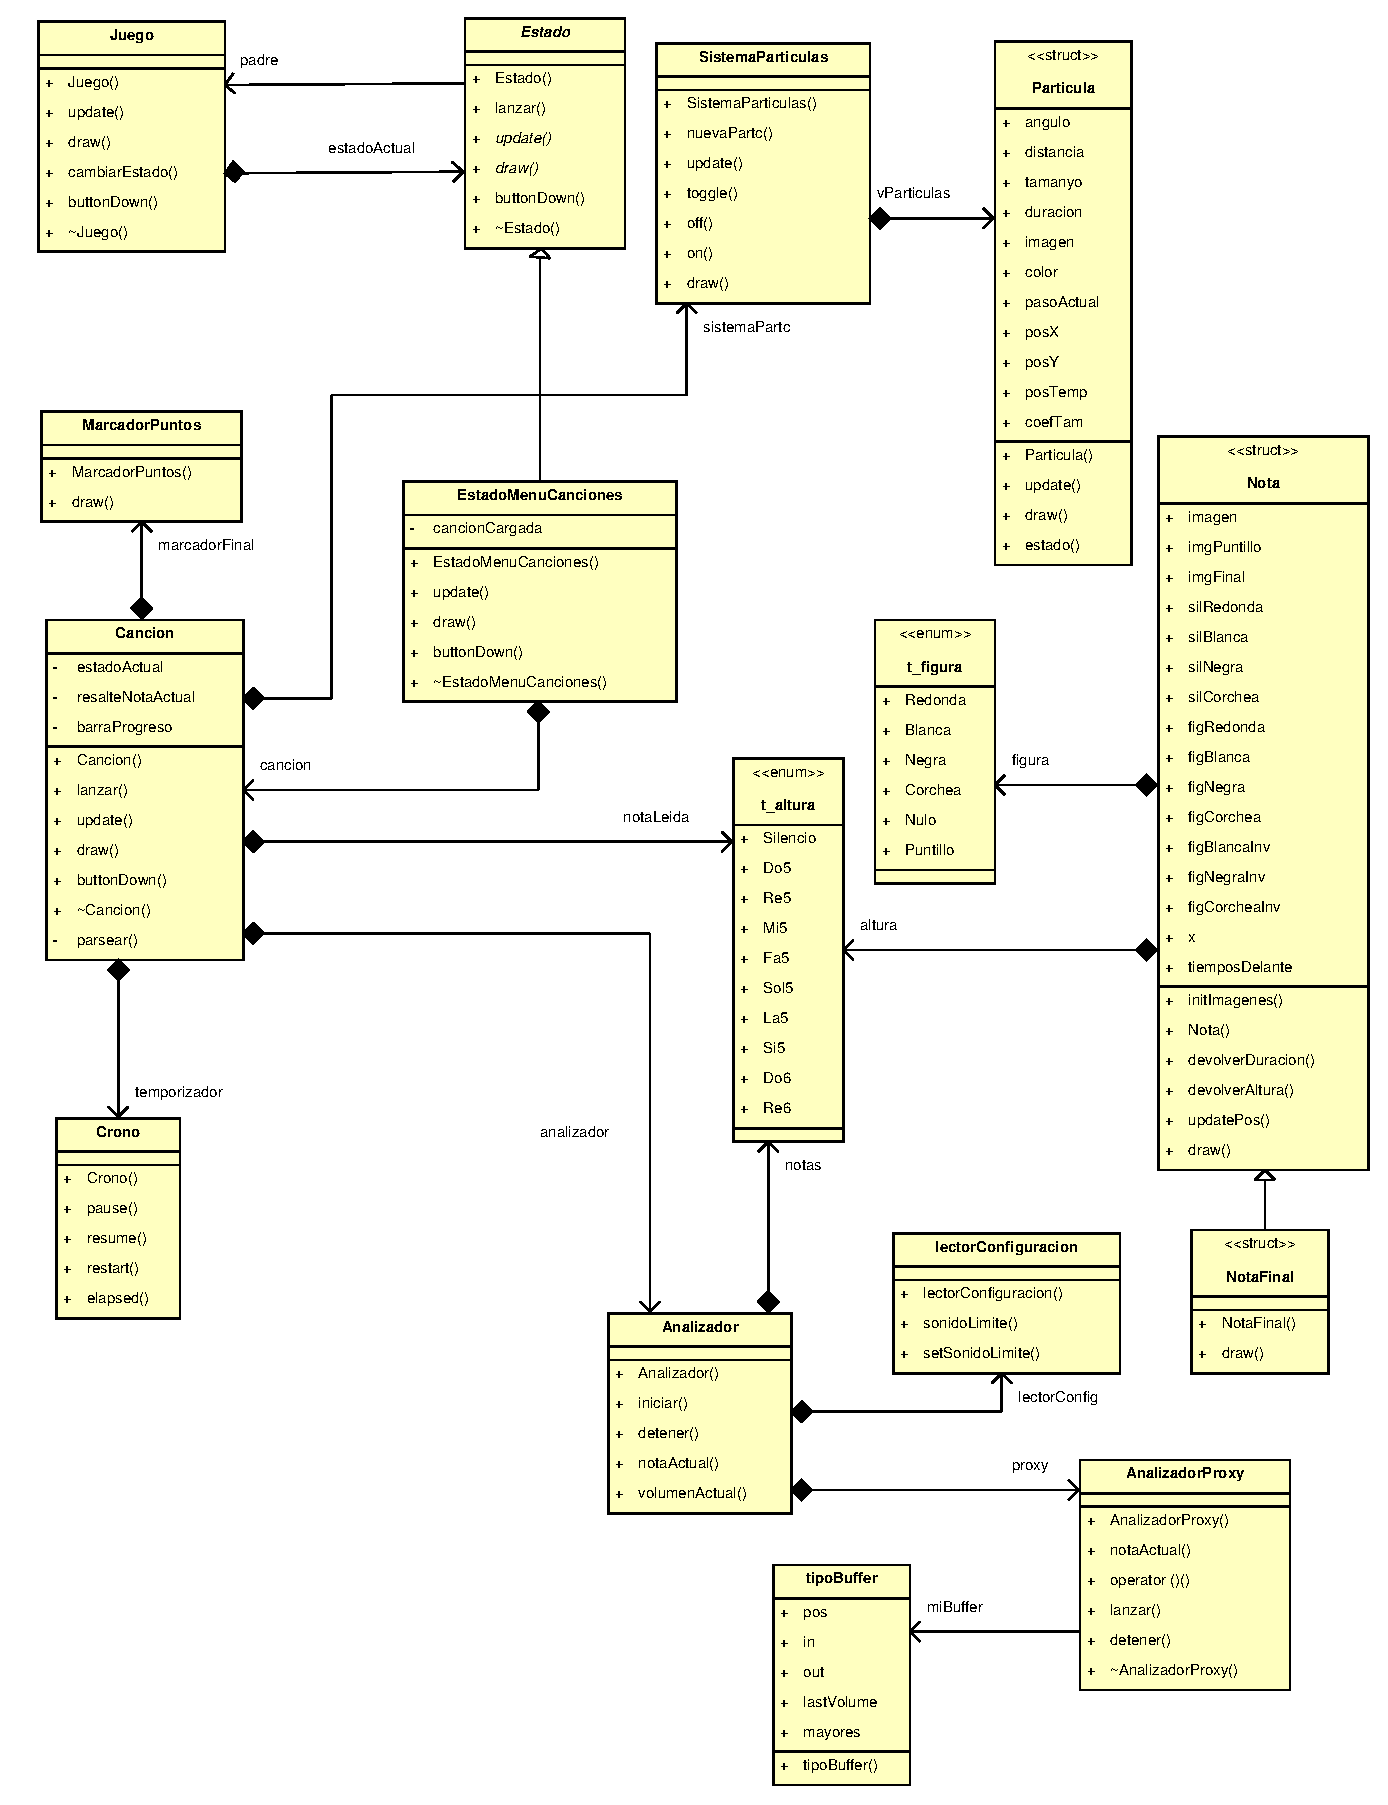
\includegraphics[width=\textwidth, clip=true, trim=0cm 0cm 0cm 0cm]{5_diseno/diagrama3}
  \caption{Diagrama de clases de diseño, parte III}
  \label{fig:diagrama_clases_3}
\end{figure}

\begin{figure}[htp!]
  \centering
  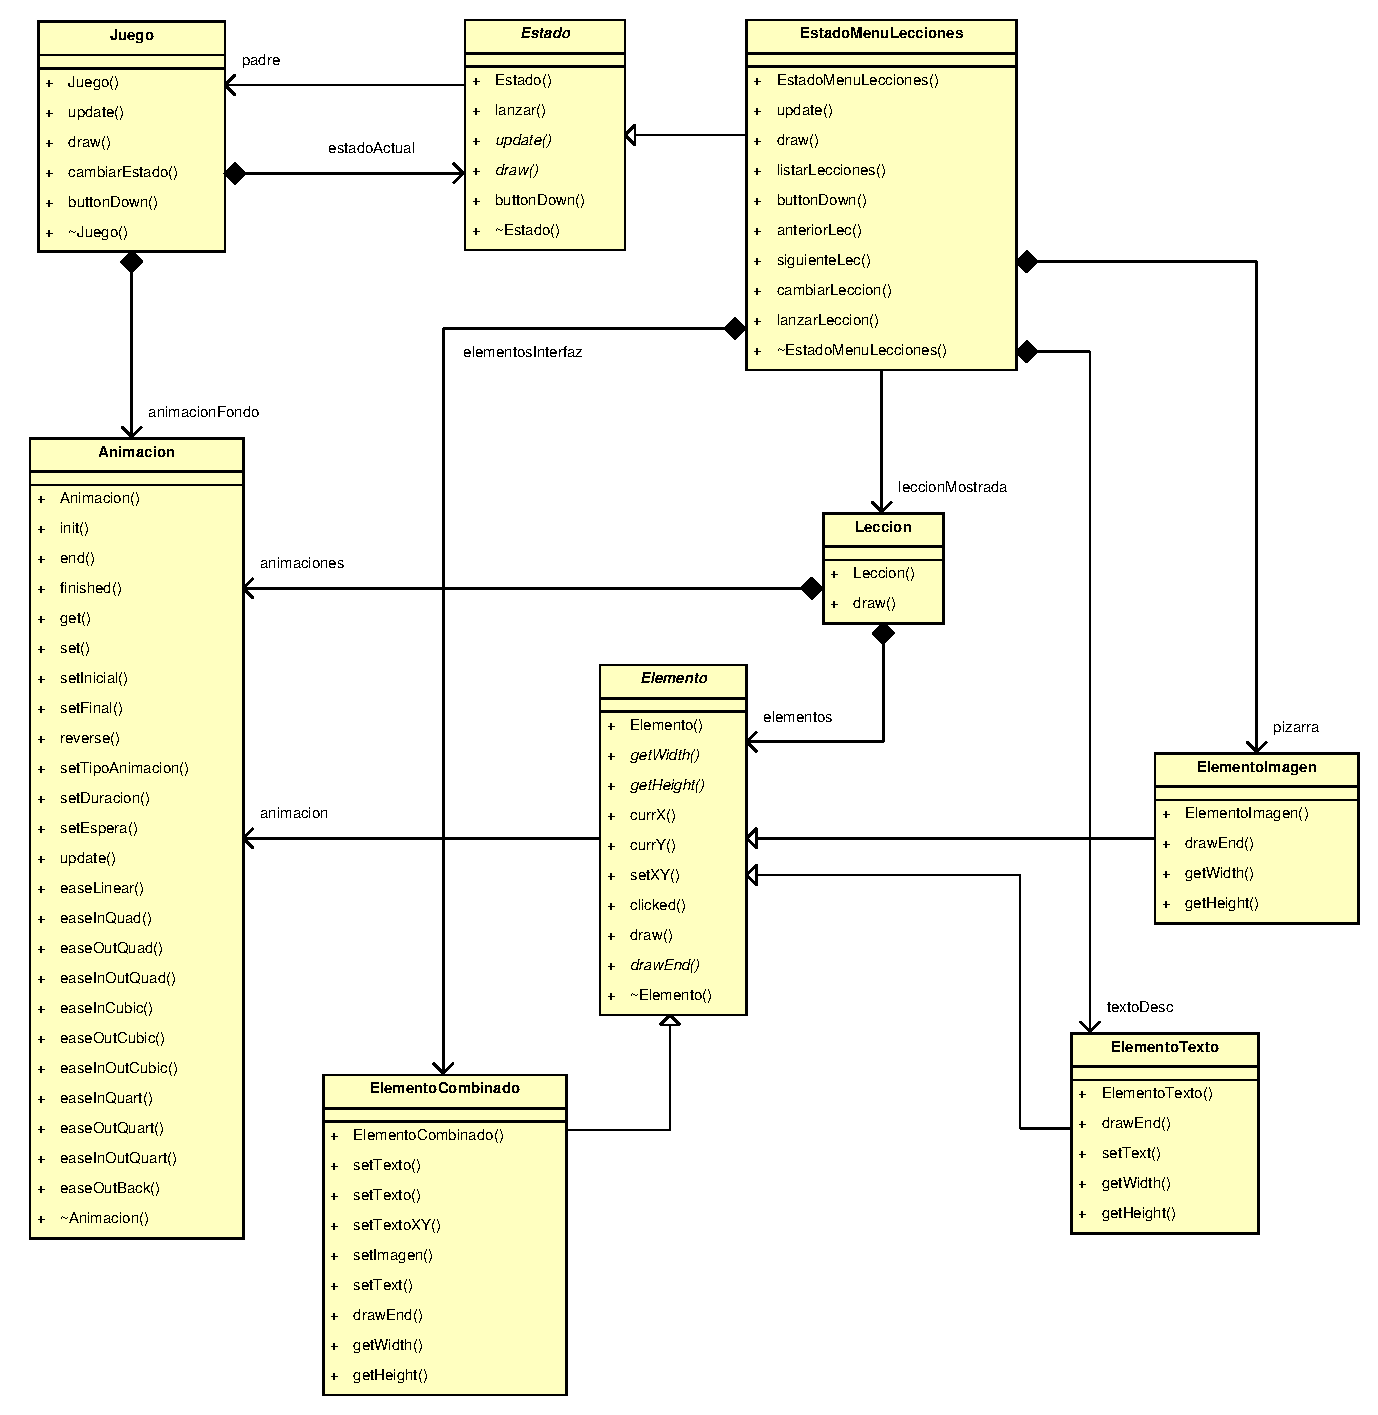
\includegraphics[width=\textwidth, clip=true, trim=0cm 0cm 0cm 0cm]{5_diseno/diagrama4}
  \caption{Diagrama de clases de diseño, parte IV}
  \label{fig:diagrama_clases_4}
\end{figure}

\section{Diseño visual}
Teniendo muy presente que el público objetivo de \textbf{oFlute} es joven y
dinámico, el diseño visual del proyecto intentó adaptarse a lo que la audiencia
podría considerar más atractivo. Desde el inicio se fijaron ciertas premisas o
\textit{guías de branding} para oFlute, que se siguieron a rajatabla a la hora
de diseñar cada uno de los elementos.

\textbf{Interfaces limpias y minimalistas}. Era imprescindible que las
interfaces gráficas de cada una de las secciones tuviera un diseño limpio y
cuidado, manteniendo en el mínimo la cantidad de elementos a mostrar en pantalla
sin descuidar el diseño.

Para conseguirlo, se optó por utilizar un fondo blanco con un sutil patrón gris
claro, que se mantiene a lo largo de todas las secciones. Un gran ejemplo de esto
es la imagen de los títulos de crédito del juego.

\begin{figure}[htp!]
  \centering
  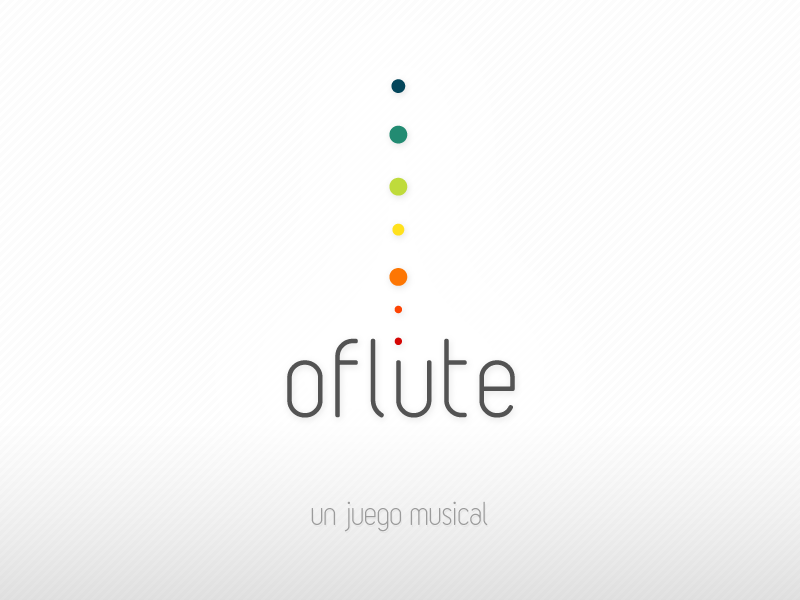
\includegraphics[width=0.7\textwidth]{apendice_manual_usuario/imagen_estadoIntro}
  \caption{Imagen de títulos de crédito de oFlute}
\end{figure}

\textbf{Paleta de colores pastel}. Para acompañar al blanco limpio de los
fondos de la interfaz se ideó una paleta de colores amplia, basado en tonos
brillantes, cercanos a pastel. Esta paleta está presente tanto en el logotipo de
oFlute, como en el resto de secciones. En especial, el menú principal se
benefició enormemente del uso de esta paleta de colores en los botones de las
secciones.

\begin{figure}[htp!]
  \centering
  
\includegraphics[width=0.8\textwidth]{5_diseno/imagen_escala_colores}
  \caption{Detalle de la paleta de colores de oFlute}
\end{figure}

\textbf{Logotipo}. A la hora de diseñar el logtipo, se hizo un
\textit{brainstorming} inicial en busca de conceptos relacionados con el
proyecto: notas musicales, flautas, pentagramas, claves de sol, etcétera.

Finalmente, decidimos utilizar el concepto de la flauta a través del espacio
negativo que genera dibujar solo los orificios de la misma, manteniendo el
tamaño original de los mismos.

\begin{figure}[htp!]
  \centering
  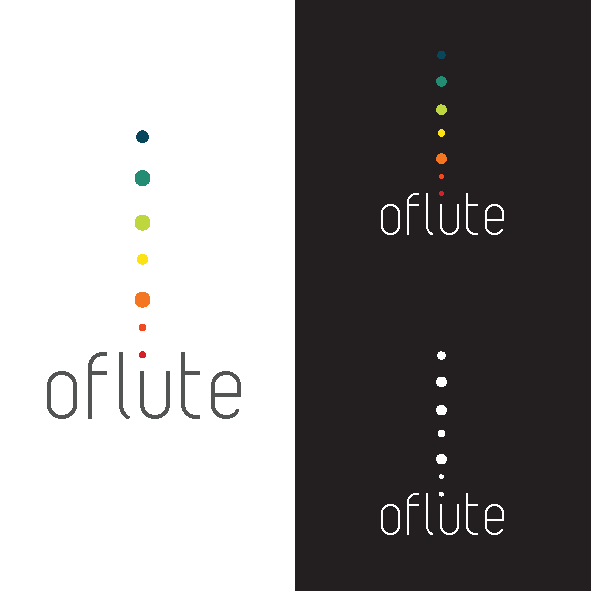
\includegraphics[width=\textwidth]{5_diseno/imagen_composite}
  \caption{Logotipo de oFlute original sobre blanco, sobre negro y en blanco y
    negro}
\end{figure}

\textbf{Tipografía}. Para adecuarse al diseño minimalista propuesto, se buscaron
tipografías simples y limpias. Para el logotipo se usó la fuente 232 MKSD
Round~\cite{fuentelogo}, y para los textos de la aplicación se usó la fuente
Miso~\cite{fuentetexto}.

%%% Local Variables: 
%%% mode: latex
%%% TeX-master: "../memoria"
%%% End: 
